%%%%%%%%%%%%%%%%%%%%%%%%%%%%%%%%%%
% HTWK Leipzig LaTeX Vorlage - Belegarbeit
%
% Das Dokument basiert teilweise auf den Vorlagen von :
% Markus Voerkel
% https://de.overleaf.com/latex/templates/thesis-template-for-hochschule-fur-technik-wirtschaft-und-kultur-leipzig/nqpftcjmmtts
%
% Linda Vogel & Jon Arnt Kårstad
% https://www.overleaf.com/latex/templates/template-projekt-htwk/mphqwccfvvwy
%
% HTWK Logo:
% https://www.htwk-leipzig.de/hochschule/hochschulkommunikation-marketing/corporate-design
%%%%%%%%%%%%%%%%%%%%%%%%%%%%%%%%%%
%
% Veröffentlicht unter CC BY-SA 4.0 - Lizenz
%
%%%%%%%%%%%%%%%%%%%%%%%%%%%%%%%%%%
%
% Hinweis: Ordner für Abbildungen, PDFs etc. müssen eigenhändig erstellt werden, da die Vorlage bei der Veröffentlichung keine leeren Ordner enthalten kann !
%
%%%%%%%%%%%%%%%%%%%%%%%%%%%%%%%%%%

%---------------------------------------
%	Dokumentenklasse
%---------------------------------------

\documentclass[
english,
toc=flat,
toc=chapterentrywithdots,
captions=tableabove,
listof=entryprefix,
listof=leveldown,
fontsize=12pt,
numbers=noenddot,
headsepline]
{scrreprt}

%---------------------------------------
%	Laden von Paketen
%---------------------------------------

\usepackage{babel}
\usepackage{lmodern}
\usepackage[T1]{fontenc}
\usepackage{float}
\usepackage{ragged2e}
\usepackage{listings}
\usepackage{subcaption}
\usepackage{listings}
\usepackage{verbatim}
\usepackage{longtable}
\usepackage{afterpage}
\usepackage{multirow}
\usepackage[T1]{fontenc}
\usepackage[table]{xcolor}

\lstset{
    language=Bash,        
    basicstyle=\ttfamily,             % Моноширинный шрифт
}

\lstdefinestyle{courier12}{
    language=Python,          % Указываем язык (но без подсветки)
    basicstyle=\ttfamily\fontsize{12}{14}\selectfont, % Courier 12 pt
    breaklines=true,          % Перенос строк
    tabsize=4,                % Размер табуляции
    commentstyle=,            % ОТКЛЮЧАЕМ стиль комментариев (чтобы они были как основной текст)
    keywordstyle=,            % ОТКЛЮЧАЕМ стиль ключевых слов
    stringstyle=,             % ОТКЛЮЧАЕМ стиль строк
    numbers=none,             % ОТКЛЮЧАЕМ номера строк
    frame=none                % Убираем рамку
}

% Geoemetry %
\usepackage{geometry}
\geometry{
	top = 27.5mm,
	headsep = 5mm,
	left = 28mm,
	right = 20mm, 
	bottom = 25mm,
	}
	
\usepackage[letterspace=150]{microtype}
\usepackage[onehalfspacing]{setspace}
	
% Caption %
\usepackage[labelfont={bf,sf},font={bf}, labelsep=space, singlelinecheck=off]{caption} 

\captionsetup[figure]{justification=centering,format=plain}
\captionsetup[table]{justification=raggedright}

% BibLaTeX %
\usepackage[
    backend=biber,
    style=numeric-comp,
    sorting=none,
    defernumbers=true
]{biblatex}
\addbibresource{References.bib}

\usepackage{csquotes}
\usepackage{amsmath}
\usepackage{graphicx}

% Hyperref %
\usepackage{hyperref}
\hypersetup{ 
    colorlinks=true,
    linkcolor=black,
    urlcolor=blue,
    citecolor=black}

%Einfacher Umgang mit Einheiten%
\usepackage{siunitx}
\sisetup{
    locale=UK,
    per-mode=fraction,
    group-minimum-digits = 6,
    group-digits = integer
}

% Bessere Kompatibilität der Dokumentenklasse mit div. Paketen %
\usepackage{scrhack}

%---------------------------------------
%	Weitere Konfigurationen
%---------------------------------------

%Anpassung der Kopf- und Fusszeile
\usepackage[autooneside=false]{scrlayer-scrpage}
\clearpairofpagestyles
\setkomafont{pageheadfoot}{\footnotesize}
\ohead{\pagemark}
\automark{chapter}
\ihead{\headmark}

%Konfiguration Verzeichnisse
\BeforeStartingTOC[toc]{\singlespacing} 
\BeforeStartingTOC[lot]{\renewcommand\autodot{:}}
\BeforeStartingTOC[lof]{\renewcommand\autodot{:}}

%Anpassung der Kapitelüberschrift
\renewcommand*{\chapterpagestyle}{scrheadings}
\RedeclareSectionCommand[%
beforeskip=0pt,
afterskip=16pt,
afterindent = false,
font=\LARGE]{chapter}

%Verhindere Zeilenumbruch innerhalb \cite[Seite]{quelle}
\renewcommand*{\prenotedelim}{\addnbspace}
\renewcommand*{\postnotedelim}{\addcomma\addnbspace}
\renewcommand*{\multicitedelim}{\addcomma\addnbspace}
\renewcommand*{\extpostnotedelim}{\addnbspace}
\renewcommand*{\volcitedelim}{\addcomma\addnbspace}
\renewcommand{\arraystretch}{1.3}

%%%%%%%%%%%%%%%%%%%%%%%%%%%%%%%%%%%%%%%%%%%%%%%%%
%
%       Bitte hier die eigenen Daten eingeben
%       (für Generierung der Titelseite etc.)
%
%%%%%%%%%%%%%%%%%%%%%%%%%%%%%%%%%%%%%%%%%%%%%%%%%

\newcommand{\autor}{Khadija Belnablia}% Vorname Name
%\newcommand{\mnr}{12345} % Matrikelnummer, bspw.: 12345

%%%%%%%%%%%%%%%%%%%%%%%%%%%%%%%%%% 
%
% Hier können weitere Autoren (und eine Gruppe) definiert werden. Diese können durch Anpassung der Titelseite.tex und der Erklaerung.tex berücksichtigt werden:
%
\newcommand{\autorII}{Yassine Ben Salah}% Vorname Name
\newcommand{\autorIII}{Ramón Elbal Ruíz}%
\newcommand{\autorIV}{Nadzeya Melnik}%
\newcommand{\autorV}{Shibichakaravarthy Senthil}%
\newcommand{\autorVI}{Devarsh Sheladiya}%
%\newcommand{\mnrII}{54321} % Matrikelnummer, bspw.: 54321
%
\newcommand{\gruppenr}{3}
%
%%%%%%%%%%%%%%%%%%%%%%%%%%%%%%%%%%

\newcommand{\betreuerI}{Prof. Dr. rer. nat. Christian Prause} % Name betreuender Prof

%\newcommand{\betreuerII}{Dipl.-Ing. Manuela Musteringenieur} % Name 2. Betreuer

\newcommand{\modulname}{Interdisciplinary IoT Project with Scientific Methods } % Hier den Modulnamen eingeben

\newcommand{\projektname}{M.A.R.S. Rover} % Hier den Belegtitel eingeben

%\newcommand{\datum}{01.\,12.\,2025}

% Fakultät und Studiengang:

%\newcommand{\fak}{Musterfakultät} % Eingabe der Fakultät
%\newcommand{\studiengang}{Musterstudiengang} % Eingabe des Studiengangs 

%%%%%%%%%%%%%%%%%%%%%%%%%%%%%%%%%%%
% Konfiguration des Anhangsverzeichnis
%
% weitere Informationen: https://komascript.de/comment/5578#comment-5578, mit Anpassungen
% Beispiel: https://komascript.de/comment/5609#comment-5609
%
%%%%%%%%%%%%%%%%%%%%%%%%%%%%%%%%%%

\DeclareNewTOC[%
  owner=\jobname,
  listname={Anhangsverzeichnis},% Titel des Verzeichnisses
]{atoc}% Dateierweiterung (a=appendix, toc=table of contents)
\DeclareNewTOC[%
  listname={Abbildungen im Anhang},% Titel des Verzeichnisses
  name=\noexpand\listoflofentryname,
]{alof}% Dateierweiterung (a=appendix, lof=list of figures)
\DeclareNewTOC[%
  listname={Tabellen im Anhang},% Titel des Verzeichnisses
  name=\noexpand\listoflotentryname
]{alot}% Dateierweiterung (a=appendix, lot=list of tables)

\makeatletter
\newcommand*{\useappendixtocs}{%
  \renewcommand*{\ext@toc}{atoc}%
  \scr@ifundefinedorrelax{hypersetup}{}{% damit es auch ohne hyperref funktioniert
    \hypersetup{bookmarkstype=atoc}%
  }%
  \renewcommand*{\ext@figure}{alof}%
  \renewcommand*{\ext@table}{alot}%
}
\newcommand*{\usestandardtocs}{%
  \renewcommand*{\ext@toc}{toc}%
  \scr@ifundefinedorrelax{hypersetup}{}{% damit es auch ohne hyperref funktioniert
    \hypersetup{bookmarkstype=toc}%
  }%
  \renewcommand*{\ext@figure}{lof}%
  \renewcommand*{\ext@table}{lot}%
}
\scr@ifundefinedorrelax{ext@toc}{%
  \newcommand*{\ext@toc}{toc}
  \renewcommand{\addtocentrydefault}[3]{%
    \expandafter\tocbasic@addxcontentsline\expandafter{\ext@toc}{#1}{#2}{#3}%
  }
}{}
\makeatother
 
\usepackage{xpatch}
\xapptocmd\appendix{%
  \addpart{\appendixname}
  \useappendixtocs
  \listofatocs

}{}{}

\BeforeStartingTOC[atoc]{\singlespacing} 
\BeforeStartingTOC[alot]{\singlespacing\renewcommand\autodot{:}}
\BeforeStartingTOC[alof]{\singlespacing\renewcommand\autodot{:}}%



%Ebenen im Inhaltsverzeichnis
\newcommand{\nocontentsline}[3]{}
\newcommand{\tocless}[2]{\bgroup\let\addcontentsline=\nocontentsline#1{#2}\egroup}
\KOMAoptions{toc=indented}

%Verwendung normaler "Gänsefüßchen"
\MakeOuterQuote{"}

%Kein Einzug nach Absatz
\setlength\parindent{0pt}

%-------------------------------------------------
%	Beginn des Dokuments und Einbinden der Kapitel
%-------------------------------------------------

\begin{document}

\begin{titlepage}
\begin{center}

\includegraphics[width=0.9\textwidth]{Konfigurationsdateien/THM_Logo.png} \par
%\vspace{2.5cm}
%\textsc{\LARGE Fakultät \fak} \par
\vspace{3.5cm}
\textsc{\Large \modulname} \par
\vspace{3cm}
{ \huge \bfseries \projektname} \par
\vspace{1.5cm}
%%%%%%%%%%%%%%%%%%%%%%%%%%%%%%%%%%
\renewcommand{\arraystretch}{1.5}
%Entsprechend der Anzahl der Autoren anpassen bzw. Kommentarzeichen (%) entfernen
\begin{table}[h]
\large
    \centering
    \begin{tabular}{lll}
        &
        \underline{Group \gruppenr} % Gruppennummer
        & \\
        \emph{Autors} % ggf. "Autoren"
        & \autor  \\
        & \autorII  \\
        & \autorIII \\
        & \autorIV   \\
        & \autorV  \\
        & \autorVI\\
        %...
        \vspace{-0.5cm} \\
        \emph{Supervisor} & \betreuerI %& \betreuerII 
    \end{tabular}
\end{table}
\renewcommand{\arraystretch}{1} \par
%%%%%%%%%%%%%%%%%%%%%%%%%%%%%%%%%%
\vfill
%{\large \datum}
\end{center}
\end{titlepage}
%\thispagestyle{empty}
\begin{center}
\large \lsstyle Erklärung
\end{center}
\vspace{1.5cm}
{\doublespacing
Ich versichere wahrheitsgemäß, die Belegarbeit selbständig angefertigt, alle benutzten Hilfsmittel vollständig und genau angegeben und alles kenntlich gemacht zu haben, was aus Arbeiten anderer unverändert oder mit Abänderungen entnommen wurde.}\par
\vspace{2cm}
%
%%%%%%%%%%%%%%%%%%%%%%%%%%%%%%%%%%
%Autor 1
\noindent
\begin{minipage}[t]{6.5cm}
% gepunktete Linie
\dotfill \par
% Text unter der Linie
\onehalfspacing
\autor \par
Leipzig, den \datum
\end{minipage} \par
\vspace{2.5cm}
%
%%%%%%%Mehrere Autoren%%%%%%%%
%
%%%%%% Autor 2:
\iffalse %Block wird von LaTeX ignoriert, für mehrere Autoren \iffalse entfernen
%
\noindent
\begin{minipage}[t]{6.5cm}
\dotfill \par
\onehalfspacing
\autorII \par
Leipzig, den \datum
\end{minipage} \par
\vspace{2.5cm}
%
\fi %Block wird von LaTeX ignoriert, für mehrere Autoren \fi entfernen
%%%%%%
%
%%%%%% Autor 3:
\iffalse % Block wird von LaTeX ignoriert, für mehrere Autoren \iffalse entfernen
%
\noindent
\begin{minipage}[t]{6.5cm}
\dotfill \par
\onehalfspacing
\autorIII \par
Leipzig, den \datum
\end{minipage} \par
%
\fi  %Block wird von LaTeX ignoriert, für mehrere Autoren \fi entfernen
%%%%%%%%%%%%%%%%%%%%%%%%%%%%%%
%
\clearpage

\tableofcontents
%\tocless\addchap{Abbildungs- und Tabellenverzeichnis}
\listoffigures
\pagebreak %Nach Belieben entfernen
\listoftables

%\chapter{Technologies and tools overview}
\paragraph{}This part presents an overview of technologies and tools that are used in the project.

\section{4tronix M.A.R.S. Rover}%before 2.1. 

\paragraph{}4tronix M.A.R.S. Rover is the main subject of this project. It was based on real-life NASA's Curiosity rover and has the following stats\cite{rover:assembly}:
\begin{enumerate}
  \item 6 Motors. 80 rpm 6V, N20 micro gear motors 
  \item 4 Servos. MG90S metal gear analog micro servos
  \item Total number of special PCBs: 30
  \item Length: 200mm
  \item Width: 185mm
  \item Height with Mast: 170mm
\end{enumerate}
\paragraph{}The rover is compatible with Raspberry Pi Zero or Microbit. In our case, Raspberry Pi 2 Zero was used. 
Rover's differential arm and couplers, connected to two rockers, help to maintain the main body’s side-to-side stability as either side encounters uneven terrain. This allows one to drive through a lot of obstacles.

\section{Operational system and software}%between 2. and 2.1
\paragraph{}Raspberry Pi Zero 2 was installed to control the rover. This is the main reason for using Raspberry Pi OS as an operating system \cite{pi:os}. 

\paragraph{}Raspberry Pi OS is a Debian-based operating system specifically optimized for Raspberry Pi hardware. It is recommended to use for most projects. Moreover, Raspberry Pi OS offers a variety of pre-installed software packages for programming, networking, and system management, making it a robust choice for controlling and managing the rover's functions.\paragraph{} 

Manufacturer provided the library rover.py written in Python. The library consists of functions to manipulate hardware. It also allows easy to utilize ultrasonic distance sensor on rover's most.

\section{MQTT Protocol}%move to communications part

\paragraph{}Message Queuing Telemetry Transport (MQTT) protocol is standardly used on the Internet of Things \cite{mqtt:spec}. The protocol is light-weight and based on the publisher-subscriber model. This offers good scalability and reliable message delivery.\paragraph{}

MQTT architecture has three main parts:
\begin{enumerate}
    \item Broker - server that manages message distribution.
    \item Client - devices that send or receive messages through the broker.
    \item Topics - special channels on the broker side where clients publish or read data from.
\end{enumerate}
\paragraph{}The user and the Rover don’t need to have connectivity towards each other, let alone be on the same network, they need to be able to connect to a broker and subscribe to the same topic.

\paragraph{}Communication with real-life Curiosity Rover occurs in two ways: through satellites orbiting Mars that relay information or via a direct signal from Earth to the rover's high-gain antenna. Small amounts of information or daily commands are transmitted via direct signal from the Earth. However, if a bigger portion of the information, such as images from the rover, should be sent, an intermediary is used.

\paragraph{} Implementation of MQTT simulates the way of sending information via satellite. Under these circumstances, Brocker represents a satellite, clients are the rover itself and an app.
\section{Technologies for web development}
\subsection{Express JS}
\paragraph{}Express.js is a simple and flexible web framework for Node.js that helps developers build web applications and APIs easily. It provides useful features like routing, middleware support, and template engine integration. Since it is lightweight and does not enforce a strict structure, developers can organize their projects as needed. Express.js is designed to handle multiple requests efficiently, making it fast and scalable. Because of its ease of use and powerful capabilities, it is widely used for building modern web applications and backend services \cite{expressJS:guide}.

\subsection{React JS}
ReactJS is a component-based JavaScript library designed for creating dynamic and interactive user interfaces. Developed and maintained by Facebook, it simplifies the development of single-page applications (SPAs) by focusing on performance and maintainability. ReactJS uses a virtual DOM to optimize rendering and ensure faster updates. It follows a declarative approach to designing UI components, making code more readable and easier to manage. Additionally, its one-way data binding enhances application control, ensuring a predictable and efficient data flow \cite{react:geek}.

\subsection{MongoDB}%sci sourses
\paragraph{}MongoDB is a modern NoSQL database designed to handle large volumes of unstructured and semi-structured data. The database uses a document-oriented approach, storing information in flexible JSON-like Binary JSON(BSON) documents. This allows developers to manage data more dynamically and efficiently, making it ideal for applications that require scalability and agility \cite{mongodb:doc_1}.
\paragraph{}IoT devices generate diverse data. MongoDB handles this data efficiently due to its several advantages. Schemaless document storage allows users to store varied data structures without predefined schemas, which is ideal for IoT's complex data. MongoDB offers horizontal scaling and and automatic sharding, making it capable of handling large IoT datasets. Database is optimized for sensor data. All of those features make MongoDB a valuable tool for big data analysis and real-time monitoring in IoT systems \cite{mongodb:iot}. 

\newpage
\section{DHT22 Sensor}

\paragraph{}DHT22 is a humidity and temperature sensor. The main information about the sensor is represented in a table below:

\begin{table}[ht]
    \centering
    \renewcommand{\arraystretch}{1.3} % Optional: Adjusts row height for better readability
    \begin{tabular}{|p{5cm}|p{7cm}|} % p{} for left-aligned columns
    \hline
     \textbf{Power Supply}    & 3.3-6 V DC   \\ \hline
     \textbf{Output Signal}    & Digital signal via single-bus   \\ \hline
    \textbf{Sensing Element}    & Polymer capacitor   \\ \hline
    \textbf{Operating Range}    & Humidity: 0-100\% RH; Temperature: -40~80°C    \\ \hline
    \textbf{Accuracy}    & Humidity: ±2\% RH (Max ±5\% RH); Temperature: <±0.5°C     \\ \hline
    \textbf{Resolution or Sensitivity}    & Humidity: 0.1\% RH; Temperature: 0.1°C    \\ \hline
    \textbf{Repeatability}    & Humidity: ±1\% RH; Temperature: ±0.2°C   \\ \hline
    \textbf{Humidity Hysteresis}    & ±0.3\% RH   \\ \hline
    \textbf{Long-Term Stability}    & ±0.5\% RH/year   \\ \hline
    \textbf{Sensing Period}   & Average: 2s  \\ \hline
    \textbf{Interchangeability}   & Fully interchangeable  \\ \hline
    \end{tabular}
    \caption{Characteristics of DHT22 Sensor}
    \label{tab:DHT22_charac}
\end{table}

%\chapter{Assembling}
\section{Hardware assembling}
\paragraph{} Responsible team members: Devarsh Sheladiya, Shibichakaravarthy Senthil

\paragraph{} The rover came in a kit form. As mentioned earlier, it consists of motors, servos, wheels, and body details. Figures \ref{fig:Assembl1}, \ref{fig:Assembl2} and \ref{fig:Assembl3} demonstrate some of the assembling stages.


\begin{figure}[ht]
    \vspace{0.4cm}
    \centering
    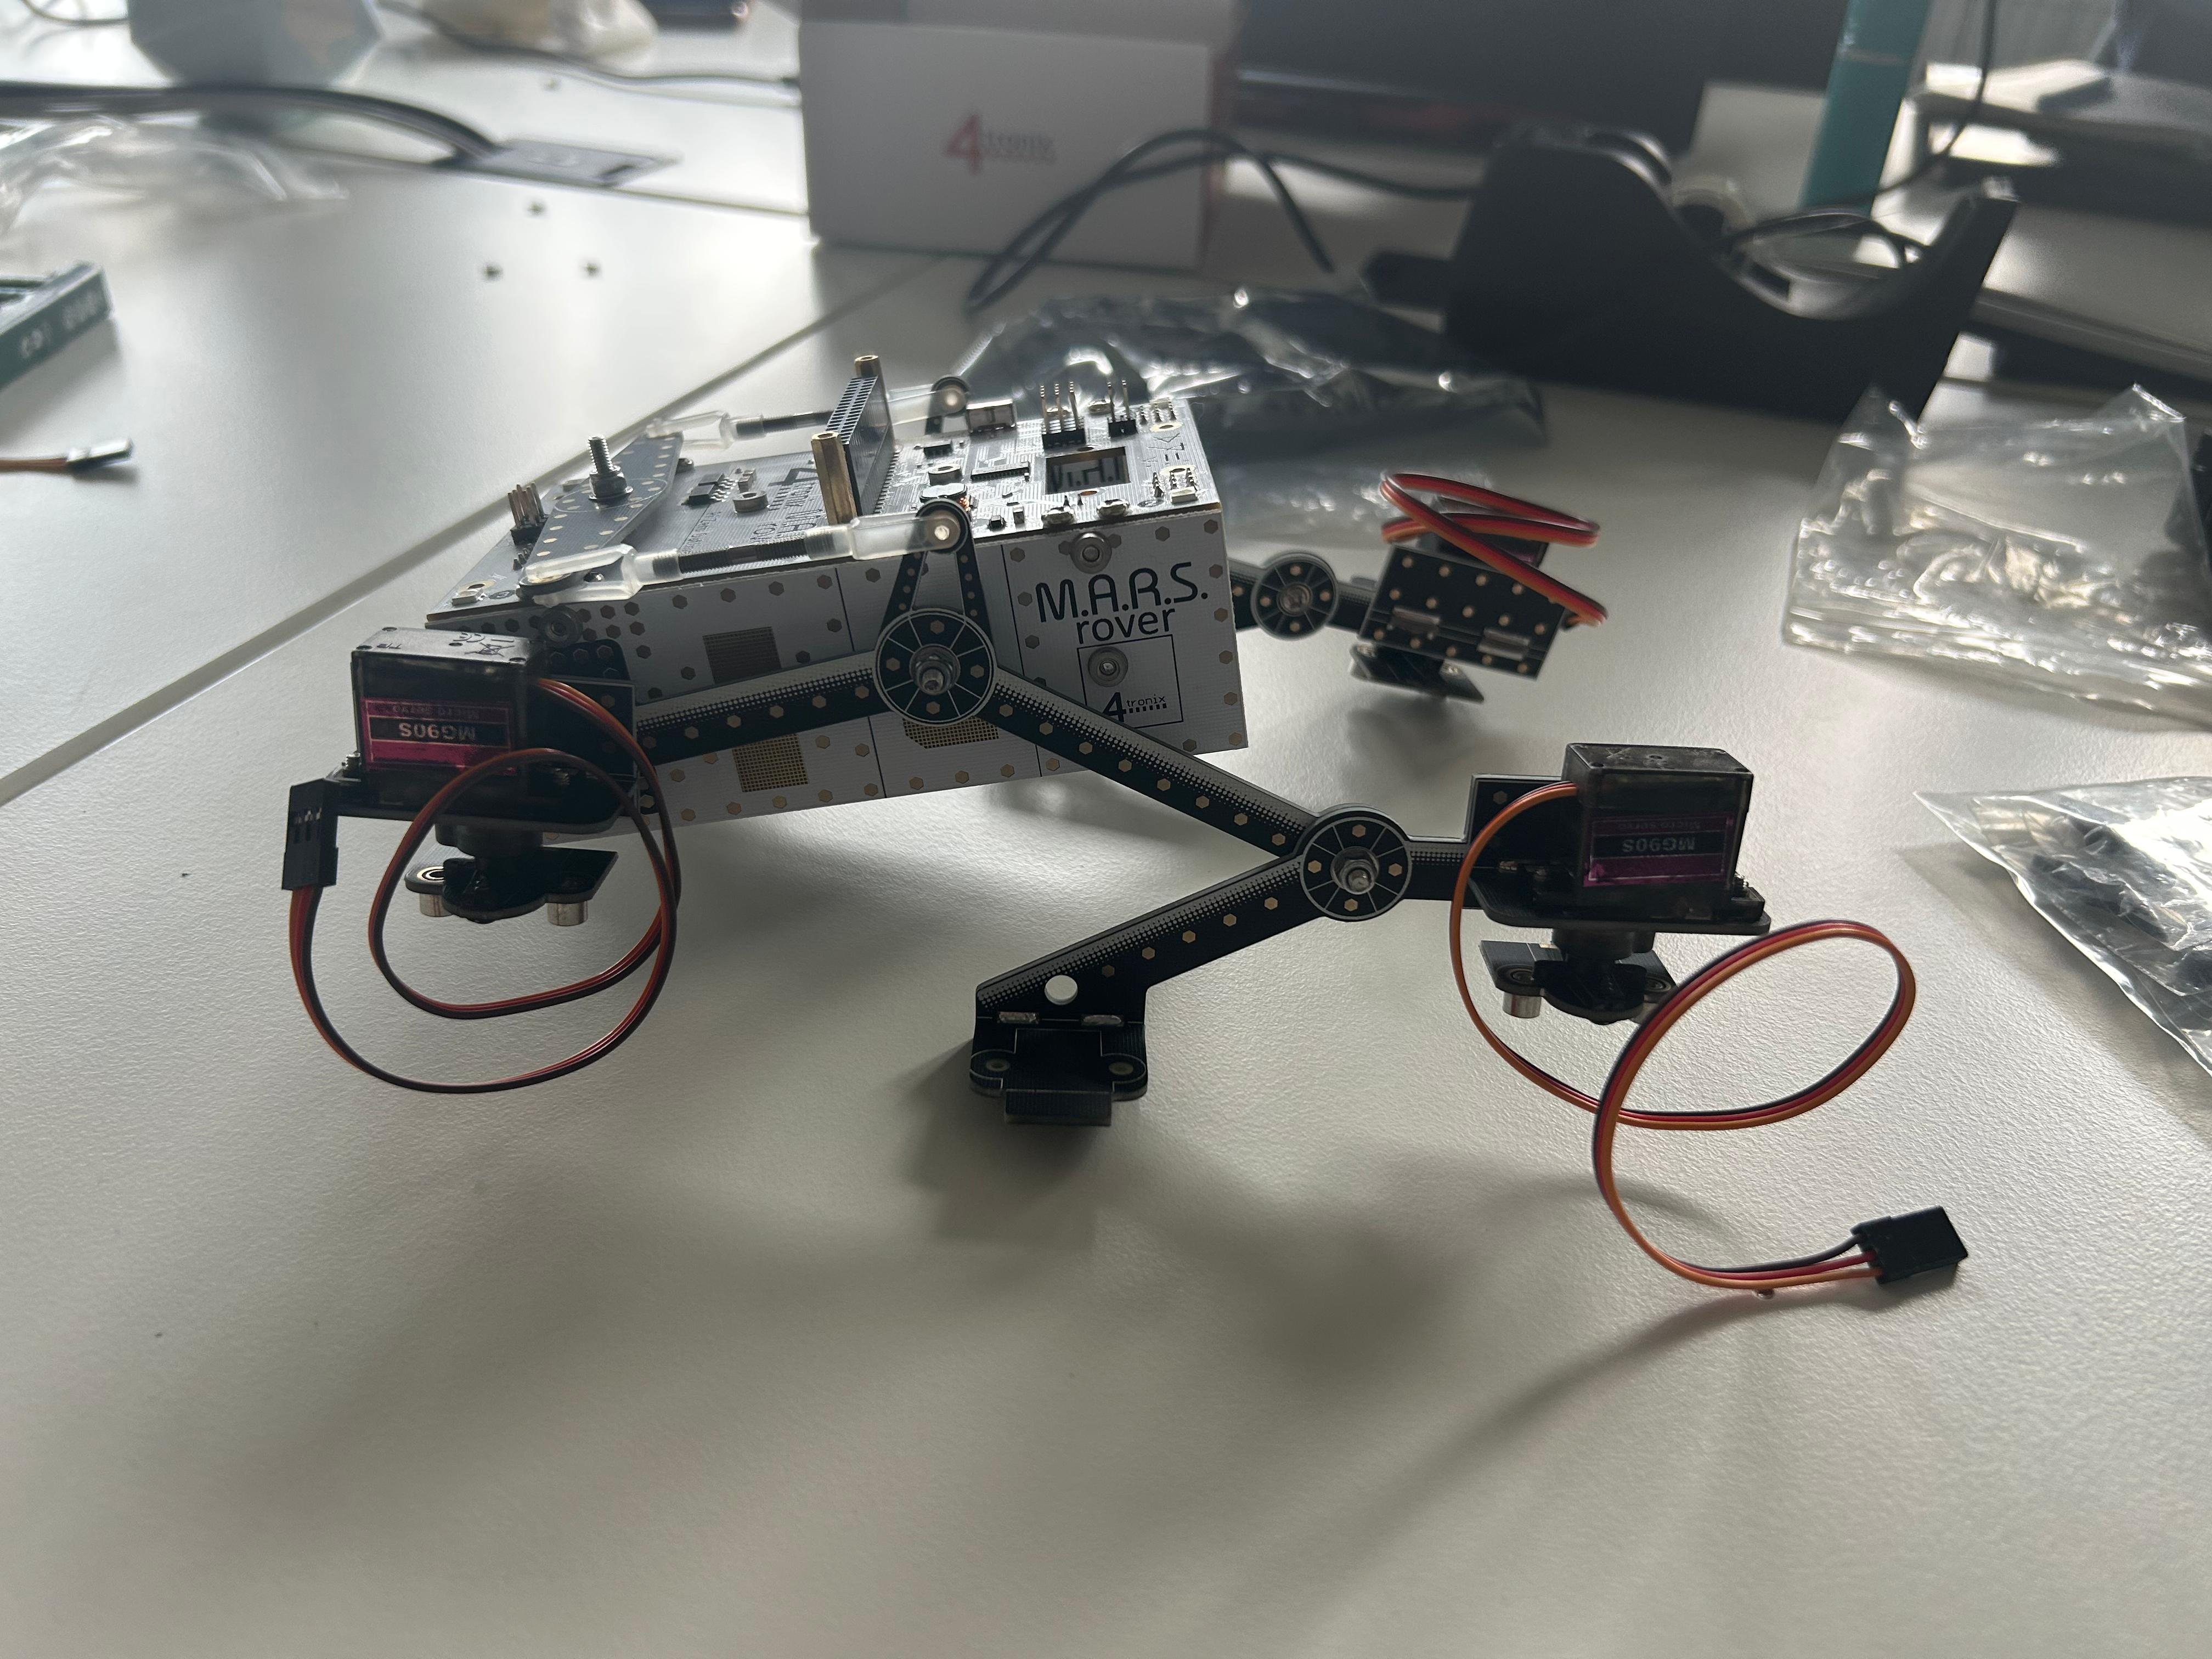
\includegraphics[width=0.48\textwidth]{Hauptkapitel/Pictures/As1.jpg}
    \caption{}
    \label{fig:Assembl1}
\end{figure}

\begin{minipage}{0.46\textwidth}
    \vspace{0.4cm}
    \centering
    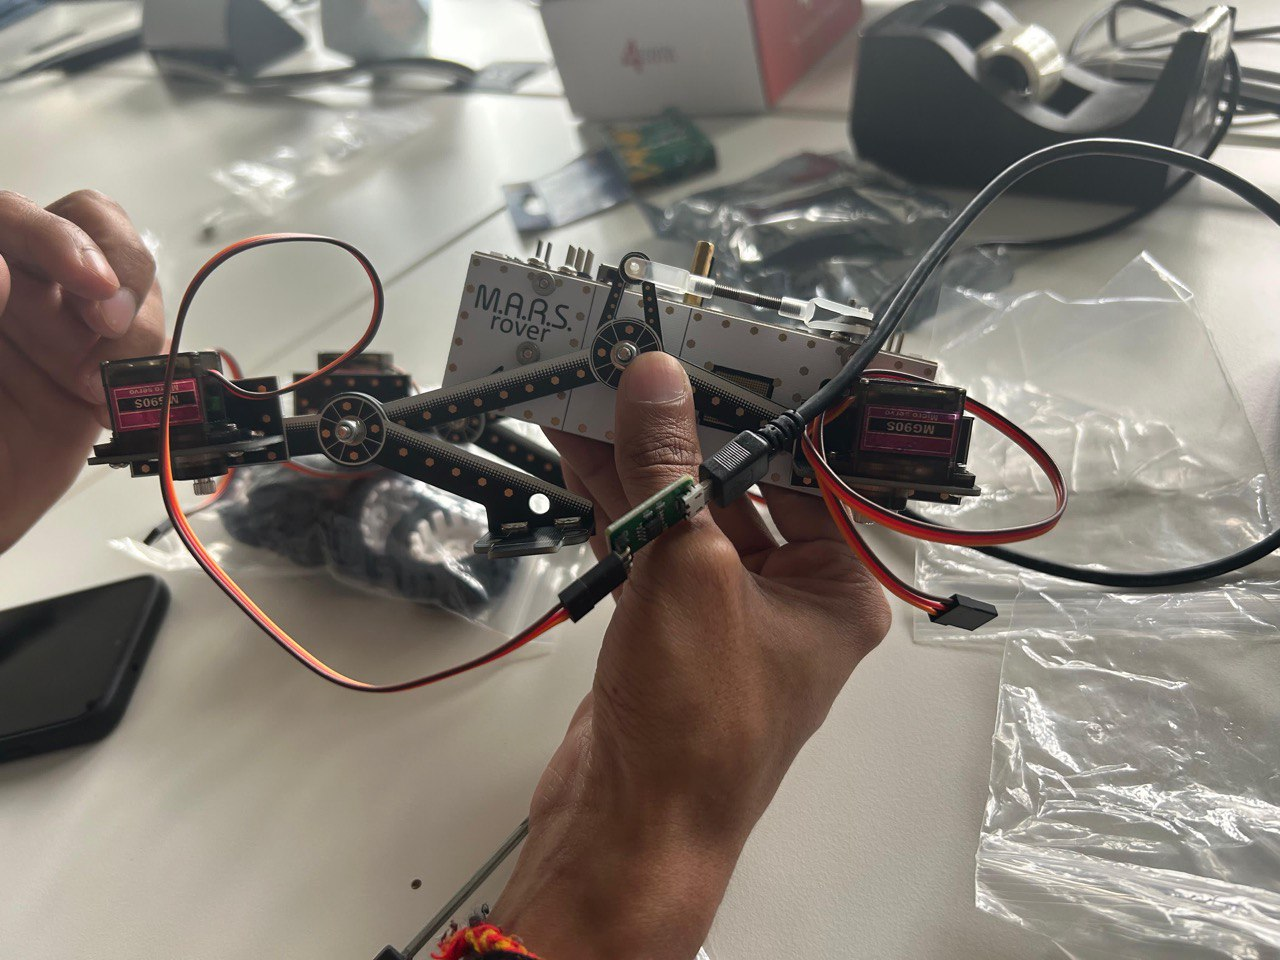
\includegraphics[width=\textwidth]{Hauptkapitel/Pictures/As2.jpg}
    \captionof{figure}{}
    \label{fig:Assembl2}
\end{minipage}
\hfill
\begin{minipage}{0.46\textwidth}
    \vspace{0.4cm}
    \centering
    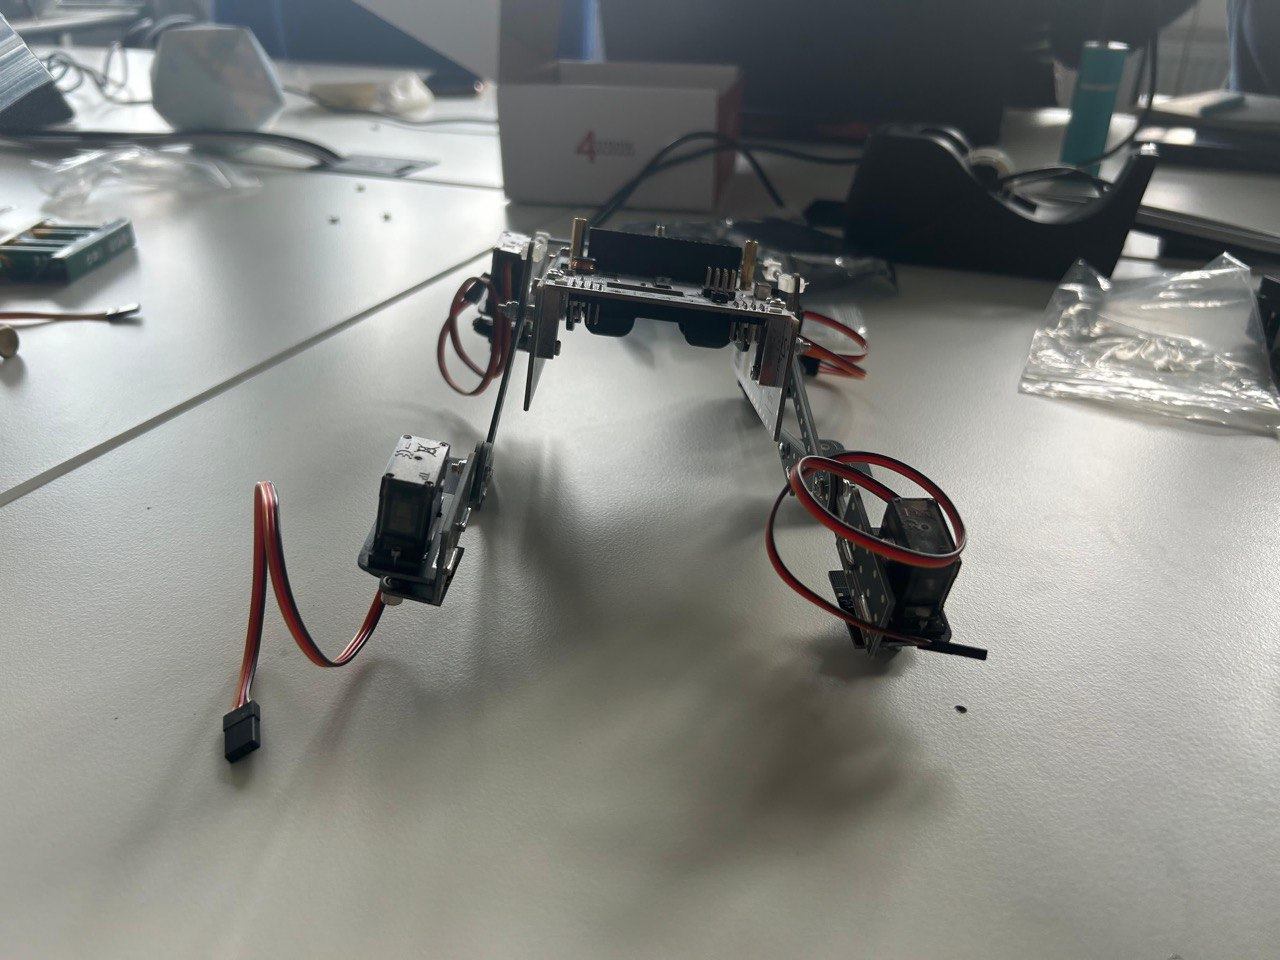
\includegraphics[width=\textwidth]{Hauptkapitel/Pictures/As3.jpg}
    \captionof{figure}{}
    \label{fig:Assembl3}
\end{minipage}

\paragraph{}Once the hardware assembly was completed, preliminary tests were conducted to verify that all components were functioning correctly. This included checking motor movement and sensor readings.

\section{Camera installation}

\paragraph{}The original Curiosity Rover has 17 cameras on board, which was the biggest number used in such a project \cite{nasa:camera}. The rover uses them to take pictures of the Mars environment.  
\paragraph{} To increase the project's potential it was decided to install a camera on the rover. The mast has a special place where the camera can be installed and it is perfectly adjusted for Raspberry Pi Camera Module 3 that was provided for our project. The figure \ref{fig:cam_rover} below demonstrates installed camera. 
 \begin{figure}[h]
     \vspace{0.4cm}
     \centering
     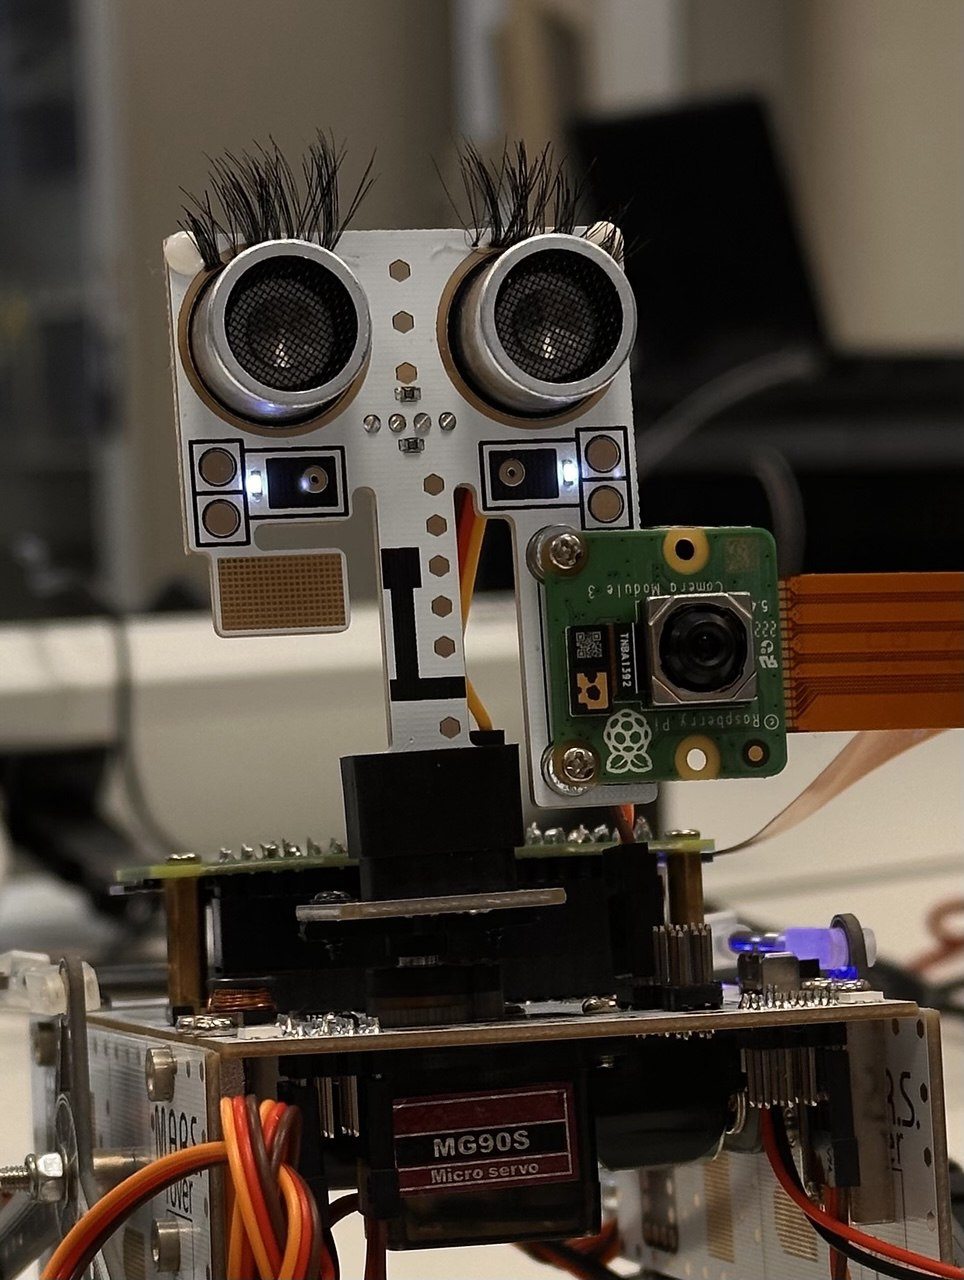
\includegraphics[width=0.4\linewidth]{Hauptkapitel/Pictures/Camera_modul.jpg}
     \caption{Installed Camera Module}
     \label{fig:cam_rover}
 \end{figure}
 
\section{DHT 22 Sensor}

\paragraph{} DHT 22 Sensor has two constructional holes that could be used to attach it to the rover. However, due to the limitations of the rover body, there were only four points of attachment: 4 holes in the corners which originally were made for the keypad. Two in the front were not the best decision, as it would limit the mast's mobility, so the sensor was installed in the back.


%\chapter{Rover Software}
\section{Configuring Raspberry Pi}
\paragraph{}The first step of configuration is installation of the Raspberry OS onto the provided SD card. During installation process connection to the phone’s Wi-Fi hotspot was preconfigured, as connecting to eduroam needed more steps in the system itself. For remote terminal access, SSH was enabled.
Before the whole rover was assembled, tasks on the  Raspberry Pi were performed with the help of an external monitor and micro USB power block. When the whole system was assembled, rover's batteries powered the circuit. 
\paragraph{}SSH protocol was used to enable the necessary interfaces for the rover, as well as the built-in Virtual Network Computing (VNC) server. VNC is a software that allows remote control of the Raspberry Pi’s desktop without other peripherals. 

\subsection{Connection via SSH}
\paragraph{}Both Raspberry Pi and the computer must be connected to the same network.The host is formed by the username and the IP address of the board. 
\paragraph{} The most convenient way to utilize SSH connection is via an additional client program. For this reason, MobaXTerm application was used. MobaXterm provides a user-friendly interface that simplifies remote access to the Raspberry Pi \cite{mobxterm:main}. Additionally, MobaXterm supports SFTP, enabling easy file transfer between the local computer and the Raspberry Pi via the built-in file explorer. Another helpful feature is a build-in text editor that is more efficient during coding. 

\subsection{Connection to eduroam network}
\paragraph{} Connection to eduroam on Linux could be done through a configurator program or manually. Due to the performance issues related to the currently installed on Raspberry Pi web browser, our team had to find alternatives that didn’t rely on it, such as downloading the eduroam configuration script externally and then uploading it to the board via mobaXTerm. The network configuration was done manually. File \lstinline|wpa_supplicant.conf| holds the information of all known networks. The following adjustments were made in this file: 

\begin{lstlisting}
 network={
        ssid="eduroam"
        scan_ssid=1
        key_mgmt=WPA-EAP
        eap=PEAP
        identity="youridentity@thm.de"
        password="yourpassword"
        phase1="peaplabel=0"
        phase2="auth=MSCHAPV2"
}
\end{lstlisting}

\paragraph{}Where \lstinline|youridentity| would be substituted with any valid THM user identifier and \lstinline|yourpassword| would be the corresponding user’s net password.
After a reboot, Raspberry Pi was connected successfully as shown on figure \ref{fig:edu_connect}:
\begin{figure}[h]
     \vspace{0.4cm}
     \centering
     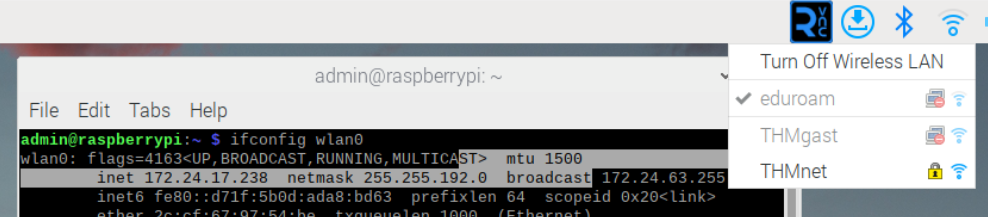
\includegraphics[width=0.9\linewidth]{Hauptkapitel/Pictures/edu_connect.png}
     \caption{Connection to eduroam}
     \label{fig:edu_connect}
 \end{figure}

\section{4tronix scripts for the rover}
\paragraph{}4tronix provides a ready to use scripts for the rover. Most of them are for testing and calibration of the hardware \cite{rover.prog:doc,}. The scripts were obtained from official site of 4tronix via the command \lstinline|wget https://4tronix.co.uk/rover.sh -O rover.sh|. \lstinline|rover.sh| script installs Python libraries and scripts. Their functionality is described in the following table \ref{tab:rv_scripts}.
\newpage
\begin{table}[h]
    \centering
    \begin{longtable}{|l|p{10cm}|}
        \hline
        \textbf{Script} & \textbf{Functionality}\\
        \hline
        \lstinline|calibrateServos.py| & Ensures that the wheels are all pointing in the correct direction. Used for testing servos. \\
        \hline
        \lstinline|rover.py| & The main library module. Consists of functions to manipulate hardware. \\
        \hline
        \lstinline|motorTest.py| & Demonstrates driving the motors. \\
        \hline
        \lstinline|servoTest.py| & Demonstrates controlling the servos. The second script for testing servos. \\
        \hline
        \lstinline|ledTest.py| & Flashes all LEDs through Red, Green, Blue and White. \\
        \hline
        \lstinline|sonarTest.py| & Shows the distance in cm for an obstacle using the ultrasonic distance sensor mounted on the mast head. \\
        \hline
        \lstinline|keypad.py| & Shows the numeric value of each key pressed on the optional keypad. \\
        \hline
        \lstinline|driveRover.py| & Basic driving program using the arrow keys to steer and move. \\
        \hline
    \end{longtable}
    \caption{Scripts provided by 4tronix}
    \label{tab:rv_scripts}
\end{table}
\vspace{-10mm}
\paragraph{}As it is mentioned in the table \ref{tab:rv_scripts},  \lstinline|rover.py| is the core component for a development. Based on this library a script \lstinline|driveRovermqtt.py| was developed to control the rover. 

\section{\lstinline|driveRovermqtt.py| script}
\paragraph{}\lstinline|driveRovermqtt.py| script contain main functionality of the rover. It also controls communication with MQTT broker. Communication side of the project will be explained in later chapters.

\subsection{Rover configuration and motion control}
\subsection{Rover hardware configuration}
\paragraph{} The following variables allow to configure the rover. 
\begin{lstlisting}[style=courier12]
# Rover Configuration
SERVO_FRONT_LEFT = 9
SERVO_REAR_LEFT = 11
SERVO_FRONT_RIGHT = 15
SERVO_REAR_RIGHT = 13
SERVO_MAST = 6
SERVO_TEMPHUM = 25

DEFAULT_SPEED = 60
INACTIVITY_TIMEOUT = 10  # Stop rover if no command received in 10 sec.
DEGREE_STEP = 15  # Mast rotation step
RECONNECT_DELAY = 5  # Delay before reconnecting MQTT after a failure
TEMPERATURE_HIGH_THRESHOLD = 30 #Upper temperature threshold
TEMPERATURE_LOW_THRESHOLD = 0 #Lower temperature threshold
HUMIDITY_THRESHOLD = 80
\end{lstlisting}
\vspace{-5mm}
\paragraph{} Variables \lstinline|RECONNECT_DELAY| and \lstinline|INACTIVITY_TIMEOUT| are important safety features. They help to deal with lost connection. Variables \lstinline|TEMPERATURE_HIGH_THRESHOLD|,\lstinline|TEMPERATURE_LOW_THRESHOLD| and \lstinline|HUMIDITY_THRESHOLD| are used for the functionality of the DHT 22 sensor.
\paragraph{} The main function for controlling the movement is \lstinline|move_rover()|.
\begin{lstlisting}[style=courier12]
def move_rover(key):
    global speed
    global client
    actions = {
        'w': move_forward,
        's': move_reverse,
        'd': turn_right,
        'a': turn_left,
        ' ': reset_servos,
        'q': lambda: rotate_mast(1),
        'e': lambda: rotate_mast(-1),
        'b': stop_rover,
        'p': lambda: publish_photo(client), #Photo task is run on a background thread to prevent stopping the system
        't': taylorSwiftmode,
    }
    if key in actions:
        actions[key]()
    elif key in {'.', '>'}:
        speed = min(100, speed + 10)
        print(f"Speed increased to {speed}")
    elif key in {',', '<'}:
        speed = max(0, speed - 10)
        print(f"Speed decreased to {speed}")
    else:
        print(f"[WARNING] Unknown command received: {key}")
\end{lstlisting}
\paragraph{}The function gets commands from an MQTT client stream and orchestrates the movement. Movement functions are based on the methods from \lstinline|rover.py| library.   

\subsection{MQTT client}
\paragraph{} For the MQTT implementation, the library \lstinline|paho.mqtt.client| was used. The rover connects to the MQTT broker during an initialization process through standard methods of \lstinline|paho.mqtt.client|. In addition to that, customized functions were developed.
\paragraph{} The functions to handle MQTT messages and communication are represented in a table \ref{tab:func_mqtt}.
\begin{table}[h]
    \centering
    \begin{longtable}{|l|p{10cm}|}
        \hline
        \textbf{Function} & \textbf{Functionality}\\
        \hline
        \lstinline|on_connect()| & Connects to the MQTT broker. In case of a failure, print the message about an error into the console.  \\
        \hline
        \lstinline|on_message()| & Receives and decodes the message from MQTT broker, then sends it to the function \lstinline|move_rover()| \\
        \hline
        \lstinline|on_disconnect()| & Handles the disconnection to the broker, prints the error message into the console, and stops the rover. \\
        \hline
    \end{longtable}
    \caption{Functions for MQTT protocol}
    \label{tab:func_mqtt}
\end{table}
\vspace{-10mm}
\paragraph{} The persistence of communication between the rover and the MQTT broker is a matter of safety. One of the issues that may appear is a disconnection from the network. To handle this situation, two functions for an Inactivity Timer were developed. The timer begins as soon as the connection to the broker is complete. Each time as the rover receives a command, the timer gets reset. If after 10 seconds the timer expires, the function to stop the rover executes and the rover's servos are reset to the default position.
\paragraph{}\lstinline|reset_inactivity_timer()| function resets the inactivity timer to prevent stopping the rover, while \lstinline|handle_inactivity()| stops the rover if no command is received within a timeout.

\subsection{Sensor data gathering and publishing}

While a background loop keeps the connection up, the rover will periodically read its sensors and send the readings to the MQTT broker. The library \lstinline|rover.py| implements a function that allows us to gather the ultrasound sensor's nearest reflection in centimeters. To gather information from the DHT22, we used a function implemented by the software RaspController. The reason for this is that the original Adafruit DHT python library has issues when running on a Raspberry Pi. Both methods use GPIO to send signals to the sensors and receive the result from the same ports. The following is the function used to gather temperature and humidity from the DHT22

\begin{lstlisting}[style=courier12]
def getTempHum(): # default to front sensor
    MAX_ATTEMPTS = 15
    MAX_NOT_FOUND_ATTEMPTS = 3
    dht = DHT(sensor_pin, isDht11)
    result = dht.read()
    not_found_attempts = 0
    
    # make some attempts, because someone may not be successful
    for x in range(0, MAX_ATTEMPTS):
        if result.is_valid() or not_found_attempts == MAX_NOT_FOUND_ATTEMPTS:
            break
        else:
            time.sleep(2)
            result = dht.read()
            if result.error_code == DHTResult.ERR_NOT_FOUND:
                not_found_attempts += 1
            else:
                not_found_attempts = 0
    return result.temperature, result.humidity
\end{lstlisting}

This data is then sent to the MQTT broker separated in their respective MQTT topics. These topics and their content are the following:
\begin{itemize}
    \item \lstinline|iotrover/distance|: Nearest reflection in centimeters gathered by the ultrasound sensor.
    \item \lstinline|iotrover/temperature|: Temperature gathered by the DHT22 in Celsius
    \item \lstinline|iotrover/humidity|: Humidity gathered by the DHT22 as a percentage.
\end{itemize}

Furthermore, we use the topic \lstinline|iotrover/warning| to send alerts regarding extreme temperature and humidity conditions caught by the rover. If the temperature is above or below the thresholds configured in the global variables  \lstinline|TEMPERATURE_HIGH_THRESHOLD| \newline and \lstinline|TEMPERATURE_LOW_THRESHOLD|. For humidity-related alerts, we define one threshold, \lstinline|HUMIDITY_THRESHOLD|, and automatically take a photo when it's surpassed. Below one can find the code related to these functions:

\begin{lstlisting}[style=courier12]
    def publish_sensor_data(client):
    """Continuously publishes distance, temperature and humidity sensor data every second."""
    while True:
        try:
            distance = rover.getDistance()
            temperature, humidity = rover.getTempHum()
            client.publish(TOPIC_DISTANCE, str(distance), qos=0)
            client.publish(TOPIC_TEMPERATURE, str(temperature), qos=0)
            client.publish(TOPIC_HUMIDITY, str(humidity), qos=0)
            print("Published distance data:", distance)
            print('Temp={0:0.1f}*C  Humidity={1:0.1f}%'.format(temperature, humidity))
            
            if temperature>TEMPERATURE_HIGH_THRESHOLD:
                print("WARNING: Hot temperature")
                client.publish(TOPIC_WARNING, "Hot temperature" ,qos=1)
                temp_warning=True
            elif temperature<TEMPERATURE_LOW_THRESHOLD:
                print("WARNING: Cold temperature")
                client.publish(TOPIC_WARNING, "Cold temperature" ,qos=1)
                temp_warning=True
            else:
                temp_warning=False
            
            if humidity>HUMIDITY_THRESHOLD and not humid_warning:
                print("Humidity threshold exceeded. Taking photo of body of water")
                humid_warning=True
                client.publish(TOPIC_WARNING, "Humidity threshold exceeded. Taking photo of body of water", qos=1)
                publish_photo(client)
            elif humidity<HUMIDITY_THRESHOLD:
                humid_warning=False
            
            if not (humid_warning or temp_warning):
                client.publish(TOPIC_WARNING, "", qos=1)
            
            time.sleep(1)
        except Exception as e:
            print(f"[ERROR] Failed to publish sensor data: {e}")
\end{lstlisting}

\subsection{Picture capturing}

Using the Raspberry Pi Camera Module 3 and the libcamera Python library, we can take photos on command, optimize them, and send them through MQTT. However, we have to make compromises when it comes to resolution and quality due to the limitations imposed by our hardware, the broker and the MQTT protocol.

First, we use the libcamera library to take a photo, compress it to JPEG format, save it as \lstinline|test.jpg|, fix its resolution to 640x480 and not send a preview on screen.

However, despite the result being way below the MQTT's MTU (256 MB), the image still needs further optimization. For this purpose, we use the image processing dependency Python Image Library (PIL) to further compress the image without a major compromise in quality. The result is a drastically smaller image. 

Finally, we publish our image in the topic\lstinline|photos| as binary data, following MQTT's best practice. It is ill-advised to encode it on a text format like Base64, as it will increase its size by 33\%. We will instead perform the encoding on the web application. Below it's a comparison of the size of the image as binary data, after its encoding in Base64 and after it has been optimized by PIL.
\begin{figure}[H]
    \centering
    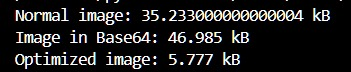
\includegraphics[width=0.5\linewidth]{Hauptkapitel/Pictures/opt_img.jpg}
    \caption{File size comparison}
    \label{fig:opt_img}
\end{figure}
The following code belongs to the function that automates the processes involved in the picture capturing and its optimization for publishing.

\begin{lstlisting}[style=courier12]
def publish_photo(client):
    """Captures and publishes a photo as base64 data MQTT message."""
    try:
        os.system("libcamera-jpeg --output \"test.jpg\" --width 640 --height 480 -n")
        foo = Image.open("test.jpg")
        foo.save('optimizedtest.jpg', optimize=True, quality=40)
        with open("optimizedtest.jpg", "rb") as image_file:
          image = image_file.read()
        print(f"Read {len(image)} bytes")
        client.publish(TOPIC_PHOTO, image, qos=2)
        print("Photo successfully sent.")
    except FileNotFoundError:
        print("[ERROR] test.jpg not found.")
    except Exception as e:
        print(f"[ERROR] Failed to publish photo: {e}")
\end{lstlisting}



 



 


%\chapter{Rover Controller Application}

\section{Overview} 
In order to provide an accessible, user-friendly interface to control the rover remotely, a web application has been developed. This application implements a back-end built with Express.js and a front-end with ReactJS.

\section{Front-end}
The front-end is the application's interface. In it, the user can control the rover and access information from it. It's main pages are the dashboard and the gallery.
\subsection{Dashboard}
In the dashboard, the user can interact with the rover and receive data from its sensors, using an MQTT client to control all data flows.
As soon as the dashboard is rendered, an MQTT client will be initiated and connected to the broker, then it will subscribe to all topics mentioned previously that the rover uses to send data.

The following image \ref{fig:web_dash} shows the implemented dashboard.
\begin{figure}[h]
    \centering
    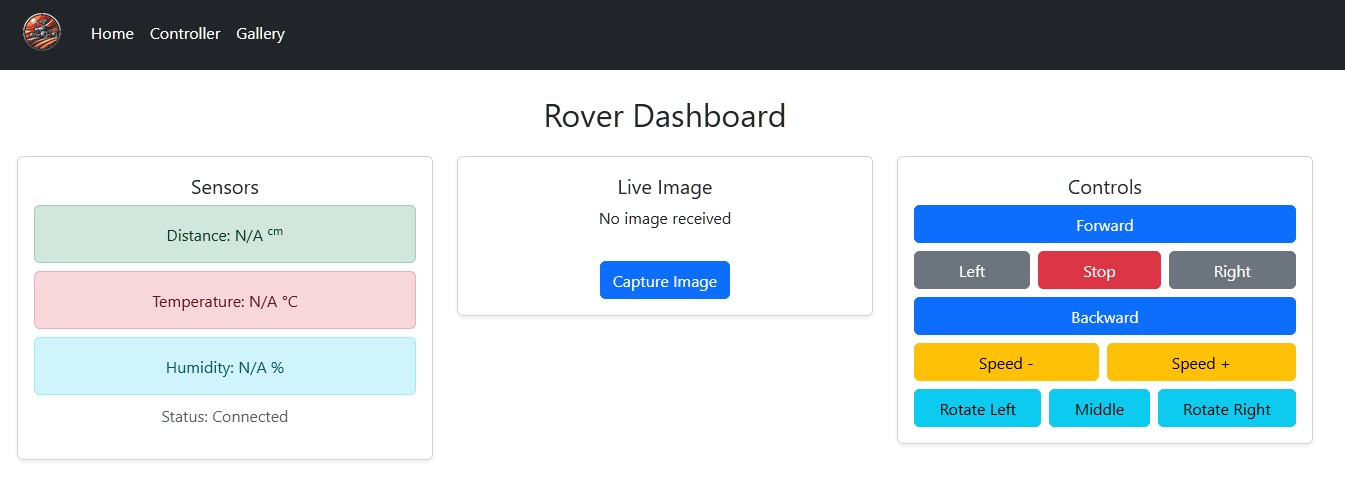
\includegraphics[width=1\linewidth]{Hauptkapitel/Pictures/App_dashboard.jpg}
    \caption{Rover's dashboard}
    \label{fig:web_dash}
\end{figure}
\paragraph{}The leftmost component shows the information gathered by the sensors, which gets updated as soon as new information gets sent and received. The middle component contains a button that publishes a command on \lstinline|iotrover/move| that makes the rover take and publish a photo through the topic \lstinline|photos|. 

%The photo will be retrieved as binary data and encoded to Base64 to show it on screen. At the same time, the image is sent to the back-end for it to be saved to the database.

The rightmost component contains a controller composed of multiple buttons. Each of these buttons will publish a command on the topic \lstinline|iotrover/move|, to which the rover is subscribed.

\subsection{Gallery}
This 
\chapter{Communication architecture}



\section{Cloud Deployment}


%\chapter{Team temesheet}

\begin{table}[h]
    \centering
    \caption{Example of a table with merged cells and separators inside cells}
    \renewcommand{\arraystretch}{1.3}  % Увеличивает высоту строк для лучшей читаемости
    \begin{tabular}{|c|p{8cm}|p{2cm}|}
        \hline
        \textbf{Team Member} & \textbf{Task} & \textbf{Time (hours)} \\
        \hline
        \multirow{3}{*}{Khadija Belnablia}  
        & Team meetings  & 9 \\
        \cline{2-3}
        & Rover Assembling   & 0,5 \\
        \cline{2-3}
        & Camera programming and image transferring & 6 \\
         \cline{2-3}
        & Analysis of different cloud platforms & 2 \\
        \cline{2-3}
         & \cellcolor{cyan}Total hours &  \cellcolor{cyan} 17,5  \\
        \hline
        \multirow{3}{*}{Yassine Ben Salah}  
        & Team meetings    & 9 \\
        \cline{2-3}
        & Rover Assembling   & 0,5 \\
         \cline{2-3}
       & Camera programming and image transferring & 5 \\
        \cline{2-3}
        & Web application development & 20 \\
         \cline{2-3}
         & \cellcolor{cyan}Total hours &  \cellcolor{cyan} 34,5  \\
        \hline
        \multirow{3}{*}{Ramón Elbal Ruíz}  
        & Team meetings    & 9 \\
        \cline{2-3}
        & Raspberry Pi Configuration & 2  \\
         \cline{2-3}
         & Rover Software Development  & 30 \\
        \cline{2-3}
         & \cellcolor{cyan}Total hours &  \cellcolor{cyan} 41  \\
        \hline
        \multirow{4}{*}{Nadzeya Melnik}  
         & Team meetings    & 9 \\
        \cline{2-3}
         & Organizational tasks    & 3 \\
        \cline{2-3}
         & Raspberry Pi Configuration & 2  \\
         \cline{2-3}
         & \cellcolor{cyan}Total hours &  \cellcolor{cyan} 15  \\  
        \hline
        \multirow{2}{*}{Shibichakaravarthy Senthil}  
         & Team meetings    & 9 \\
        \cline{2-3}
         & Rover Assembling   & 4 \\
          \cline{2-3}
         & Code optimization   & 20 \\
          \cline{2-3}
         & \cellcolor{cyan}Total hours &  \cellcolor{cyan} 33  \\
        \hline
        \multirow{2}{*}{Devarsh Sheladiya}  
         & Team meetings    & 9 \\
        \cline{2-3}
       & Rover Assembling   & 6 \\
        \cline{2-3}
         & \cellcolor{cyan}Total hours &  \cellcolor{cyan} 15  \\
        \hline
    \end{tabular}
    \label{tab:merged_cells}
\end{table}

\begin{singlespacing}
\printbibliography[
    heading=bibintoc,
    title=Bibliography
]
\end{singlespacing}

%\appendix %Entfernen/Auskommentieren um Anhang zu deaktivieren
%\chapter{Beispiel 1} %Entfernen/Auskommentieren um Anhang zu deaktivieren

\end{document}
